\begin{figure}[H]
    \centering

\begin{tikzpicture}
\pgfplotsset{
    every axis/.style={ymin=0},
    width=0.75\textwidth,
    height=0.25\textheight,
    xtick={1, 2, 3, 4, 5, 6, 7, 8},
    y axis style/.style={
    yticklabel style=#1,
    ylabel style=#1,
    y axis line style=#1,
    ytick style=#1}}
\begin{axis}[ scale only axis, ymin=0, ymax=170, xmin=1,xmax=8, axis y line*=left, xlabel=Number of Cores, ylabel=Duration (s), y axis style=green!75!black]
    \addplot[smooth, green!75!black, mark=o, draw] 
    coordinates 
    {
        (1,146.502)
        (2,95.754)
        (3,78.7675)
        (4,70.4585)
        (5,68.8315)
        (6,65.7855)
        (7,63.6405)
        (8,62.438)
    };
\end{axis}
%
\begin{axis}[ scale only axis, ymin=0, ymax=1800, xmin=1,xmax=8, axis y line*=right, axis x line=none, ylabel=DEC (j), y axis style=blue]%
    \addplot[smooth, blue, mark=x] 
    coordinates 
    {
        (1,1786.609386131)
        (2,1291.746824)
        (3,1110.7472166)
        (4,1148.809866)
        (5,1128.59226)
        (6,1101.48778)
        (7,1057.67119)
        (8,1034.65925)
    };
\end{axis}
%
\begin{axis}[red, scale only axis, ymin=0, ymax=20, xmin=1,xmax=8, axis y line*=right, axis x line=none, ylabel=DEC per second (w)]%
\pgfplotsset{every outer y axis line/.style={xshift=2cm}, every tick/.style={xshift=2cm}, every y tick label/.style={xshift=2cm} }
    \addplot[smooth, red ,mark=+] 
    coordinates 
    {
        (1,6.2209610)
        (2,9.813724)
        (3,11.79982)
        (4,14.959794)
        (5,15.45286)
        (6,16.0206841)
        (7,16.215658)
        (8,16.60837)
    };
\end{axis} 

\end{tikzpicture}
    \caption{The evolution of the DEC (blue), DEC per second (red) and duration (green) as more cores are allocated to 3DM on DUT 1}
    \label{fig:exp_3_dut_1_3dm_result}
\end{figure}